Prvi korak pri prepoznavanju rukom pisanih slova sastoji se od prikupljanja skupa podataka te obrade istoga. Obrada se sastoji od niza provedenih transformacija i filtra nad danim dokumentom, poput izdvajanja pojedinog slova, pretvaranja slike u sive nijanse, binarizacije, dilatacije, rezanja, skaliranja te stanjivanja \engl{thinning}. Cijeli postupak je prikazan na slici \ref{fig:image_process_flow}.
\begin{figure}[htb]
\centering
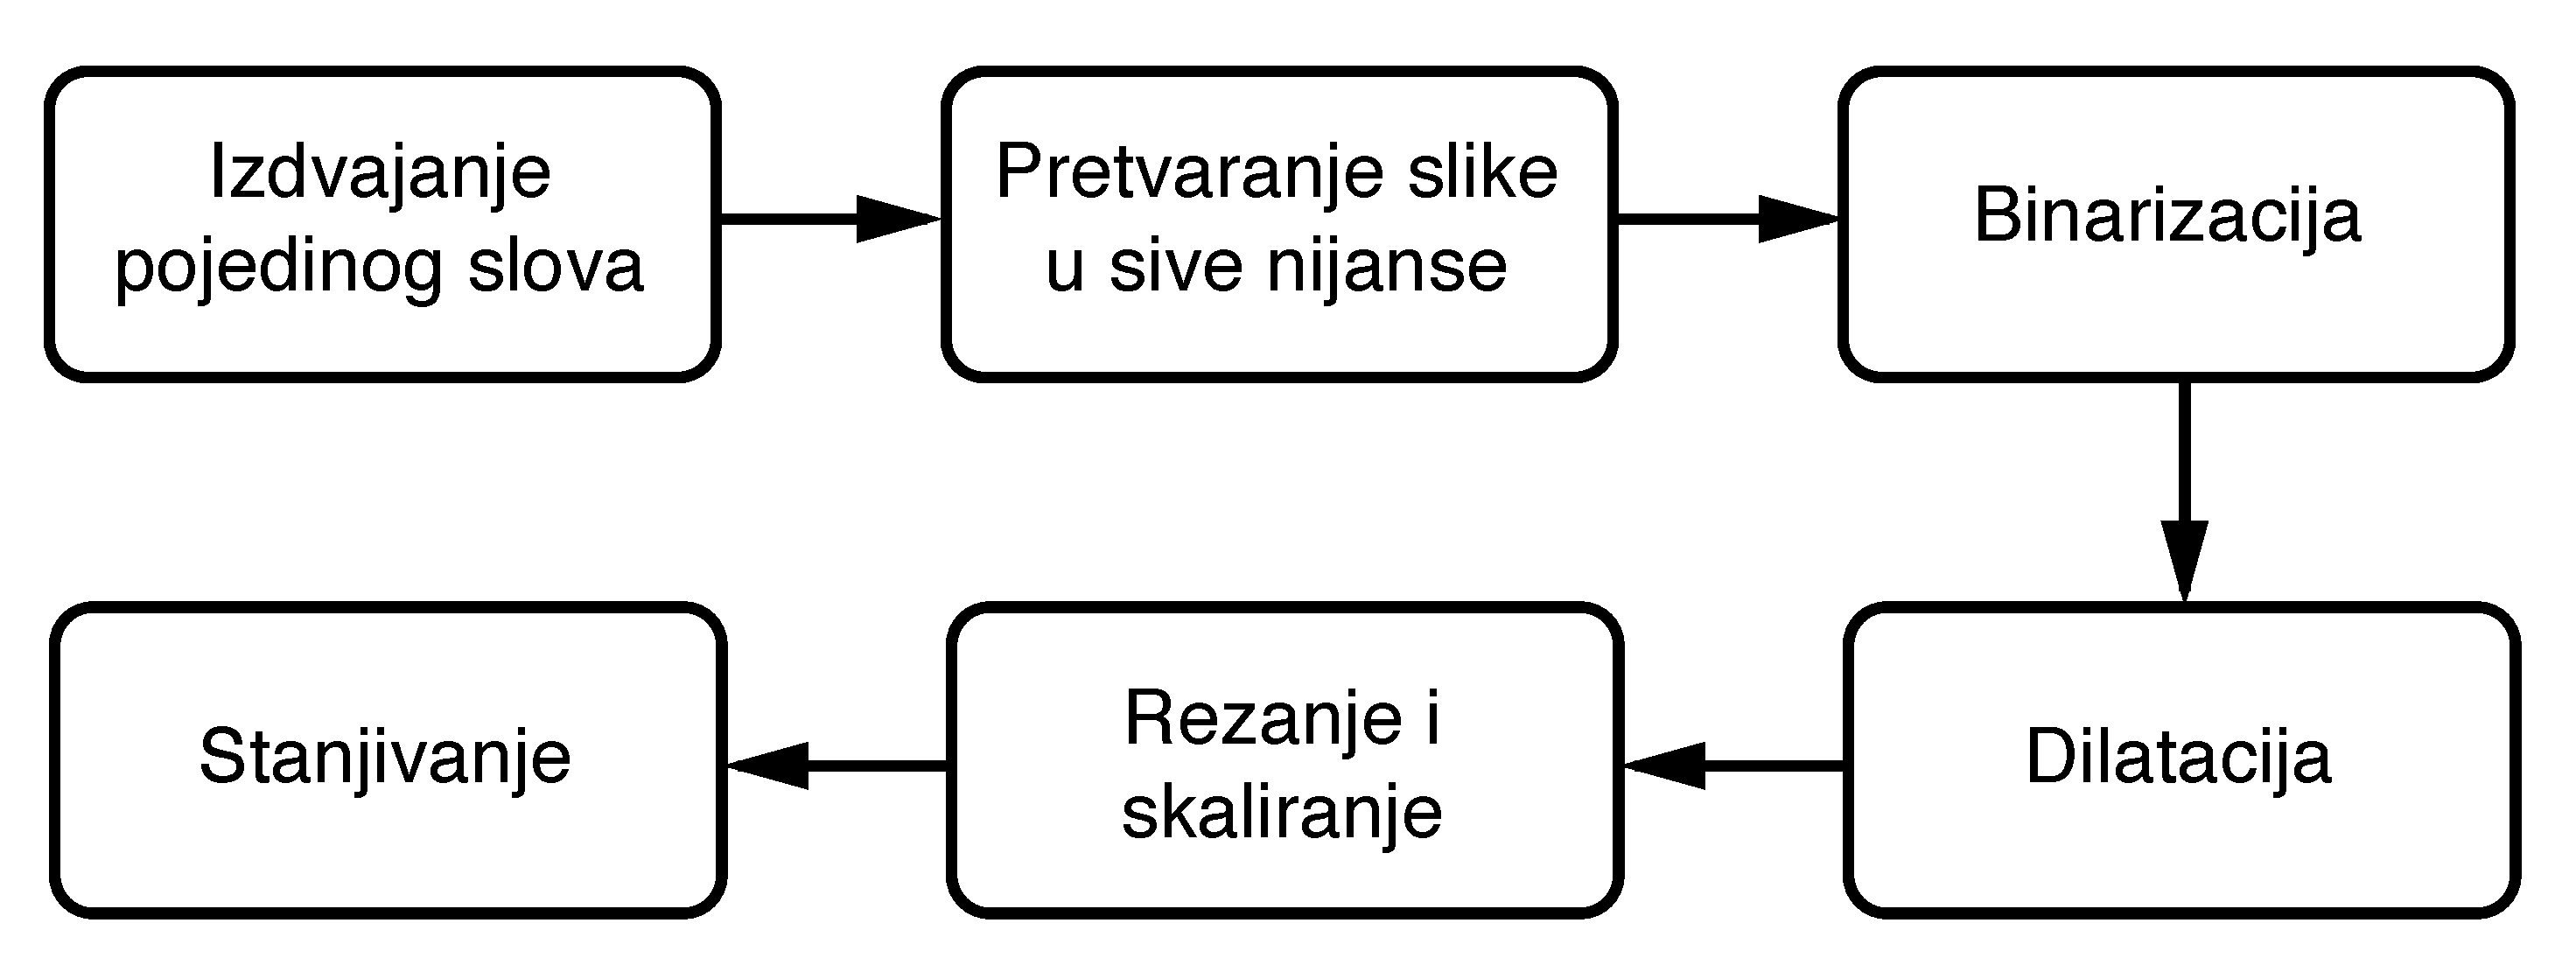
\includegraphics[width=12cm]{images/image_process_flow.pdf}
\caption{Postupak obrade slike}
\label{fig:image_process_flow}
\end{figure}

\section{Prikupljanje skupa podataka}
Prikupljanje rukom pisanih slova se obavljalo pomoću obrasca, prikazanog na slici \ref{fig:obrazac}, na kojem je trebalo ispisati po pet varijanti velikog i malog tiskanoga slova hrvatske i engleske abecede te dodatnog znaka '-' koji bi u sustavima za automatsko ocjenjivanje odgovora služio kao znak za poništavanje danog odgovora. Prostor za unos pojedinog slova je kvadratnih dimenzija kako bi se kasnije olakšalo izdvajanje pojedinog slova 
Za daljnje izdvajanje pojedinog slova iz obrasca koristio se alat \emph{Sketch}, dostupan samo za \emph{OS X} operacijski sustav. \emph{Sketch} se uglavnom koristi za razvoj dizajna za mobilne aplikacije (\emph{iOS, Android}), no za potrebe ovog rada se pokazao vrlo praktičnim jer nudi definiranje regija na slici koje je moguće sve skupa odjednom izrezati, te svaku regiju spremiti u zasebnu datoteku. Pri obradi svakog novog obrasca trebalo je samo mijenjati pozadinu, to jest obrazac, dok bi regije zadržale svoj položaj.

Za potrebe pisanja ovog rada prikupljeno je sedamnaest obrazaca, od kojih su dvoje ispisani grafitnom olovkom pa je skenirani oblik bio vrlo loše kvalitete, i jedan na ćirilici. Obrasci su skenirani u boji te su na računalu prebačeni u nijanse sive boje. Razlog tomu je loša implementacija filtra sivih tonova na skenerima, što će biti objašnjeno u sljedećem potpoglavlju.
\begin{figure}[htb]
\centering
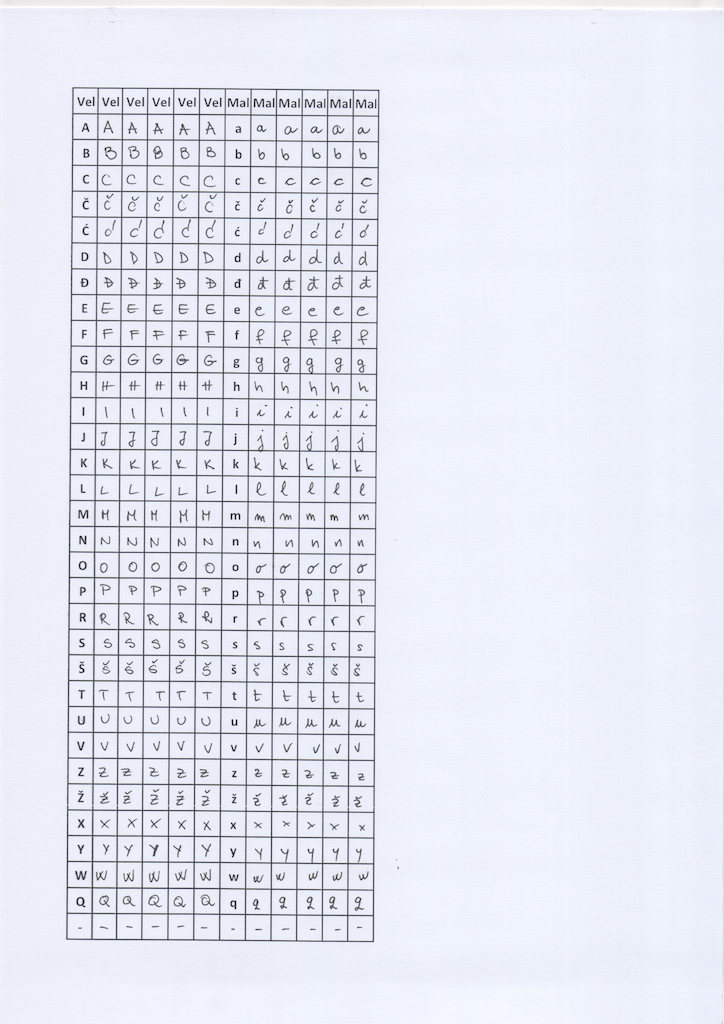
\includegraphics[width=8cm]{images/obrazac.png}
\caption{Obrazac za prikupljanje rukom pisanih slova}
\label{fig:obrazac}
\end{figure}

\section{Pretvaranje boje u nijanse sive}
Prvi korak nakon izdvajanja pojedinog slova je pretvaranje boje u nijanse sive. U svakodnevnoj uporabi se nalazi nekoliko algoritama \citep{grayscaleAlg} i većinom su vrlo jednostavni za implementirati.

Za početak nužno je shvatiti kako računalo koristi i prikazuje boje. Za prikaz boja koristi se aditivni model RGB \engl{Red Green Blue}, koji stapanjem u određenim omjerima, crvene, zelene i plave boje daje ostale boje vidljivog spektra. Tako izostanak sve tri boje, to jest prisutnost u omjeru $0:0:0$, daje crnu boju dok prisutnost svih boja u omjeru $1:1:1$ daje bijelu boju. 

Može se uočiti, ukoliko su sve tri komponente u podjednakim omjerima dobiva se boja koja se nalazi u spektru između crne i bijele boje, što je zapravo spektar sivih nijansi. Stoga se svi algoritmi za pretvorbu boja u nijanse sive temelje na pristupu gdje su sve tri komponente podjednako raspoređene.

Prvi algoritam je vrlo jednostavan i intuitivan. Siva nijansa pojedinog slikovnog elementa se dobiva tako da se boja slikovnog elementa rastavi na tri navedene komponente. Omjer pojedinih komponenti se zbraja te se uzima srednja vrijednost, kako je prikazano izrazom \eqref{eq:uniform_grayscale}.
\begin{equation} \label{eq:uniform_grayscale}
E_y = \frac{E_R + E_G + E_B}{3}
\end{equation}

Prikaz rada algoritma je vidljiv na slici \ref{fig:grayscale_uniform_example}. Algoritam je intuitivan i vrlo jednostavan, no u praksi ne daje najbolje rezultate. Problem leži u ljudskom oku i načinu na koji opaža boje. Ljudsko oko zelenu boju opaža puno jače nego crvenu, te crvenu opaža jače nego plavu.

\begin{figure}[htb]
    \centering
    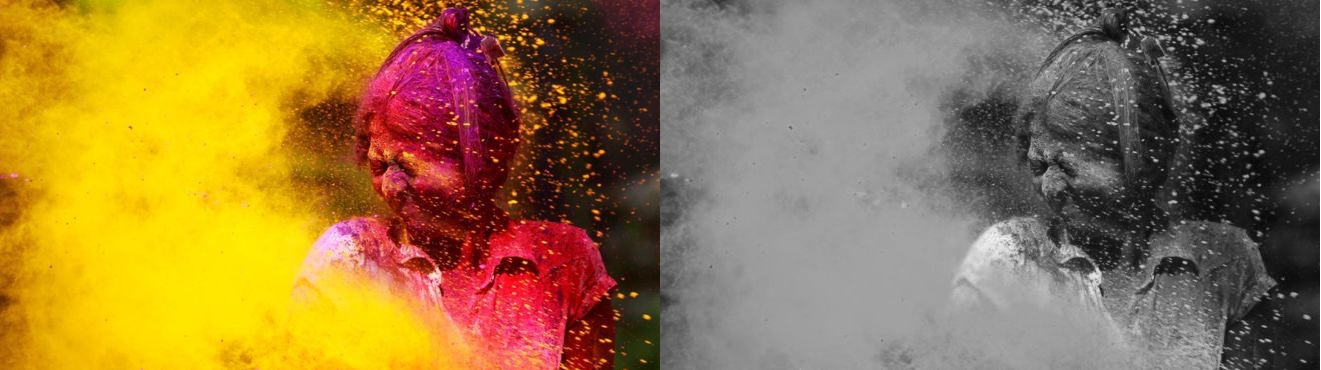
\includegraphics[width=14.5cm]{images/grayscale_uniform_example_h.jpg}
    \caption{Prikaz rada prvog algoritma pretvorbe boja u nijanse sive, preuzeto iz \citep{grayscaleImg}}
    \label{fig:grayscale_uniform_example}
\end{figure}

Na slici \ref{fig:grayscale_uniform_example}, na dijelu koji je u boji, vrlo jasno se opaža žuta boja, no pretvorbom slike u sive tonove uporabom prvog algoritma dobiva se dojam kao da se žuta boja stopila s pozadinom. Žuta boja je sastavljena od tri navedene komponente u omjeru $1:1:0$, te je predloženi algoritam zapravo u jednakom omjeru "pomiješao" zelenu i crvenu komponentu što se kosi sa načinom na koji ljudsko oko opaža boje.

Stoga intuitivno slijedi da bi zelena trebala biti najzastupljenija, zatim crvena i plava. Organizacija ITU \engl{International Telecommunication Union} u svojoj normi ITU-R BT.709-6 \citep{ITUgrayscale} predlaže drugi algoritam u kojem bi crvena komponenta imala udio s 22.16\%, zelena s 71.56\% te plava s 7.22\%, što je prikazano izrazom \eqref{eq:itu_grayscale}.
\begin{equation} \label{eq:itu_grayscale}
E_y = 0.2126E_R + 0.7152E_G + 0.0722E_B
\end{equation}

Izraz \eqref{eq:itu_grayscale} se često može naći u literaturi pod imenom \emph{Luma} te daje mnogo bolje rezultate nego izraz \eqref{eq:uniform_grayscale}. Na slici \ref{fig:grayscale_example_all} mogu se usporediti rezultati obadva izraza, gdje je jasno vidljiva prednost korištenja izraza \eqref{eq:itu_grayscale}.

\begin{figure}[htb]
    \centering
    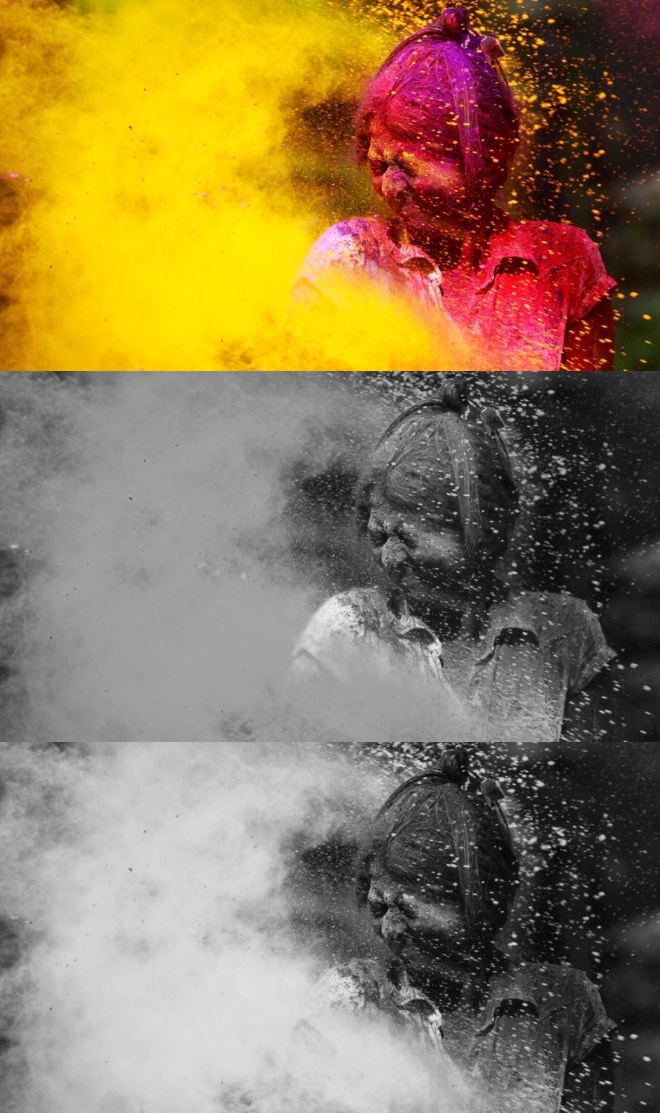
\includegraphics[width=9cm]{images/grayscale_example_all.jpg}
    \caption{Usporedba prvog i drugog algoritma pretvorbe boja u nijanse sive}
    \label{fig:grayscale_example_all}
\end{figure}

Za potrebe ovog rada korišten je izraz \eqref{eq:itu_grayscale}. Sama obrada obrasca i pretvorba u nijanse sive mogla se napravit prilikom skeniranja, no nije iz razloga što većina današnjih skenera i digitalnih kamera koristi treći algoritam koji je zapravo najjednostavnijih od svih i daje najlošije rezultate. Skener ili digitalna kamera se sastoji od senzora za pojedinu komponentu, to jest crvenu, zelenu i plavu. Pri pretvorbi boje u nijanse sive, skener ili kamera, kako ne bi trebao vršiti bilo kakvo računanje, odabire jednu komponentu i proglašava trenutnu vrijednost te komponente kao nijansu sive. U većini slučajeva je to zelena komponenta, zbog već spomenutog načina na koji ljudsko oko opaža boje.

Prikaz rada algoritma uporabom izraza \eqref{eq:itu_grayscale} nad skeniranim slovom vidljiv je na slici \ref{fig:grayscale_char_example}.

\begin{figure}[htb]
    \centering
    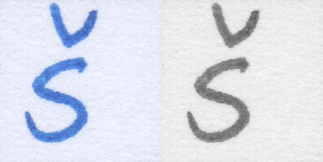
\includegraphics[width=8cm]{images/char_grayscale_example.png}
    \caption{Prikaz rada drugog algoritma nad skeniranim slovom}
    \label{fig:grayscale_char_example}
\end{figure}

Implementacija kompletnog rješenja pretvorbe slike u nijanse sive uporabom izraza \eqref{eq:itu_grayscale} u programskom jeziku \emph{Java} dana je sljedećim izvornim kodom.
\lstset{language=Java, tabsize=2}
\begin{lstlisting}
public BufferedImage applyFilter(BufferedImage sourceImage) {
        int width = sourceImage.getWidth();
        int height = sourceImage.getHeight();
        BufferedImage filteredImage = new BufferedImage(width, height, sourceImage.getType());

        int gray, rgb;
        for (int i = 0; i < width; i++) {
            for (int j = 0; j < height; j++) {
                rgb = sourceImage.getRGB(i, j);
                gray = getGray(ImageUtilities.getRed(rgb),
                        ImageUtilities.getGreen(rgb),
                        ImageUtilities.getBlue(rgb));

                gray = ImageUtilities.
                        colorToRGB(255, gray, gray, gray);
                filteredImage.setRGB(i, j, gray);
            }
        }
        return filteredImage;
    }
    
    private int getGray(int red, int green, int blue) {
        return Math.round(0.2126f * red +
                0.7152f * green +
                0.0722f * blue);
    }
\end{lstlisting}

Nakon pretvaranja boja u nijanse sive slijedi binarizacija dobivene slike slova.

\section{Binarizacija}
Binarizacija je postupak kojim se slika sivih nijansi pretvara u crno-bijelu sliku. Sam postupak binarizacije je vrlo jednostavan. Odabere se prag binarizacije, to jest vrijednost sive nijanse iznad koje će se slikovni element smatrati bijelim, a ispod te vrijednosti crnim. 

Kako bi se izbjegla ovisnost o pragu binarizacije, koristi se \emph{Otsu-ova} metoda binarizacije \citep{1979:ots}, koja prag određuje dinamički. Osnova na kojoj se temelji navedena metoda je korištenje histograma slike uz pretpostavku da slika sadrži dvije klase slikovnih elemenata, pozadinu i prednji plan, to jest u slučaju ovog rada slovo i pozadinu, kako je i prikazano na slici \ref{fig:histogram}.
\begin{figure}[htb]
    \centering
    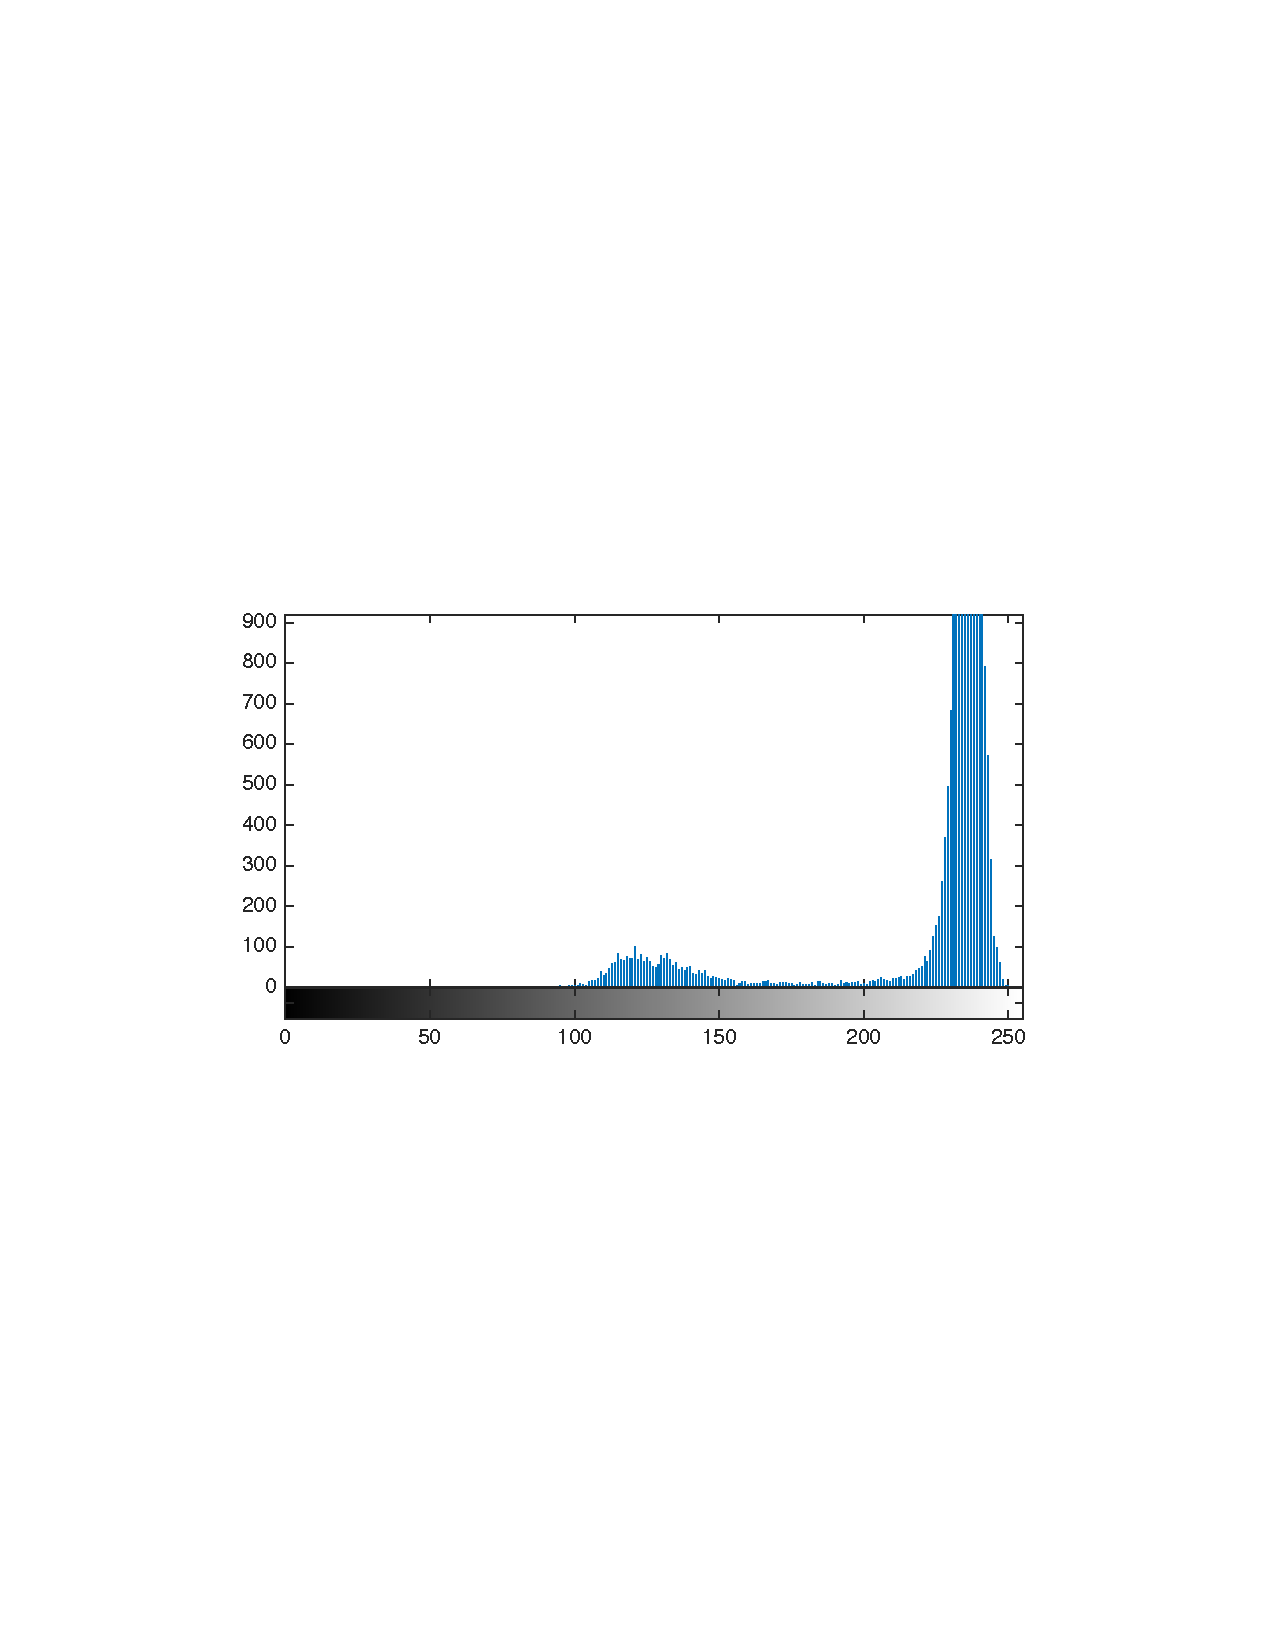
\includegraphics[width=12cm]{images/histogram.pdf}
    \caption{Histogram sive slike}
    \label{fig:histogram}
\end{figure}

Prvi korak je izračun histograma slike koji će se koristiti u daljnjim koracima. Otsu je u svojoj metodi pokazao da je klase moguće odijeliti korištenjem histograma slike i disperzije unutar i između razreda. Za svaki prag $t$ računa se disperzija unutar razreda i vrijednost pri kojoj je minimalna odabire se za prag binarizacije:
\begin{equation} \label{eq:within_class}
    \sigma_w^2(t) = \omega_0(t)\sigma_0^2(t) + \omega_1(t)\sigma_1^2(t),
\end{equation}
gdje su $\omega_0(t)$ i $\omega_1(t)$ definirane kao vjerojatnosti pojave, to jest udio prednjeg plana i pozadine:
\begin{align}
    \omega_0(t)&=\sum_{i=0}^{t-1}p(i), \label{eq:background} \\
    \omega_1(t)&=\sum_{i=t}^{L-1}p(i)=1-\omega_0(t), \label{eq:foreground}
\end{align}
ukoliko se intezitet nijansi sive boje kreće u rasponu $[0, L-1]$, a $p(i)$ predstavlja vjerojatnost pojave određene komponente $i$ u histogramu sive slike, gdje je $i \in [0, 255]$. $p(i)$ je definiran izrazom \eqref{eq:histogram_p_i}.
\begin{equation} \label{eq:histogram_p_i}
    p(i) = \dfrac{histogram(i)}{\sum_{j=0}^{L-1}histogram(j)}
\end{equation}

Računanje disperzije unutar razreda je složeno i zahtjeva mnogo računskih operacija. No maksimizacija disperzije između razreda ekvivalentna je minimizaciji disperzije unutar razreda stoga je izračun disperzije između razreda češće korišten oblik, pogotovo pri implementaciji na računalu. Matematički opisano to izgleda ovako \citep{1979:ots}:
\begin{equation} \label{eq:between_class}
    \sigma_b^2(t) = \sigma^2 - \sigma_w^2(t) = \omega_0(t)\omega_1(t)(\mu_1(t) - \mu_0(t))^2,
\end{equation}
gdje su $\mu_0(t)$ i $\mu_1(t)$ očekivanja pojedinog razreda definirana kao:
\begin{align}
    \mu_0(t)&=\sum_{i=0}^{t-1}\frac{i\cdot p(i)}{\omega_0(t)}, \label{eq:mean_bg} \\
    \mu_1(t)&=\sum_{i=t}^{L-1}\frac{i\cdot p(i)}{\omega_1(t)}, \label{eq:mean_fg}
\end{align}

Implementacija izračuna \emph{Otsu-ovog} praga u programskom jeziku \emph{Java} prikazana je sljedećim izvornim kodom.
\lstset{language=Java, tabsize=2}
\begin{lstlisting}
    private int threshold(int[] histogram, int size) {
        float sum = 0, varMax = 0, sumB = 0;
        for (int i = 0; i < 256; i++) {
            sum += i * histogram[i];
        }
        int wB = 0, wF = 0, threshold = 0;;

        for (int i = 0; i < 256; i++) {
            wB += histogram[i];
            if (wB == 0) continue;
            wF = size - wB;
            if (wF == 0) break;

            sumB += (float) (i * histogram[i]);
            float mB = sumB / wB;
            float mF = (sum - sumB) / wF;

            float varBetween = (float) wB * (float) wF * (mB - mF) * (mB - mF);
            if (varBetween > varMax) {
                varMax = varBetween;
                threshold = i;
            }
        }
        return threshold;
    }
\end{lstlisting}

Prikaz rada algoritma binarizacije uporabom Otsuove metodom otkrivanja praga prikazan je na slici \ref{fig:binarization_example}.

\begin{figure}[htb]
    \centering
    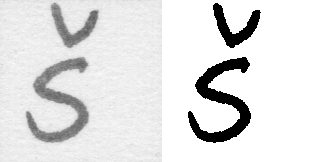
\includegraphics[width=8cm]{images/binarization_example.png}
    \caption{Prikaz rada algoritma binarizacije nad sivom slikom}
    \label{fig:binarization_example}
\end{figure}

Sljedeći korak je dilatacija binarne slike, kojeg nije nužno uvijek provesti, već ovisi o samoj kvaliteti dostupnog skupa podataka.

\section{Dilatacija}
Dilatacija je jedan od osnovnih operatora u području matematičke morfologije. Obično se primjenjuje na binarnim (crno-bijelim) slikama, no postoje i verzije algoritma koje rade i za slike sivih nijansi. Laički rečeno, dilatacija služi za podebljavanje te popunjavanje sitnih nepravilnosti i praznina unutar prednjeg plana, što može bitno utjecati na daljnju obradu slike. Matematički, dilatacija je definirana kao
\begin{equation} \label{eq:dilation}
    D(\textbf{A, B}) = \textbf{A} \oplus \textbf{B} = \bigcup_{b \in \textbf{B}} \textbf{A}_b.
\end{equation}
Skup \textbf{A} predstavlja sliku, to jest skup točaka koje pripadaju slici, nad kojom se vrši dilatacija, dok je skup \textbf{B} operator koji se naziva strukturni element, odnosno skup točaka strukturnog elementa, u literaturi često naveden pod imenom jezgra \engl{kernel}, i on je jezgra algoritma dilatacije. Strukturni element može biti raznih oblika, od kruga do kvadrata, te on određuje vrstu i svojstva dilatacije.

Za potrebe ovog rada korišten je kvadratni strukturni element dimenzija $3 \times 3$ prikazan na slici \ref{fig:kernel}. Na slici \ref{fig:kernel} oznaka '1' označava crni slikovni element. Element označen crvenom bojom predstavlja centralni element kojim se vrši usporedba s izvornom slikom.
\begin{figure}[htb]
    \centering
    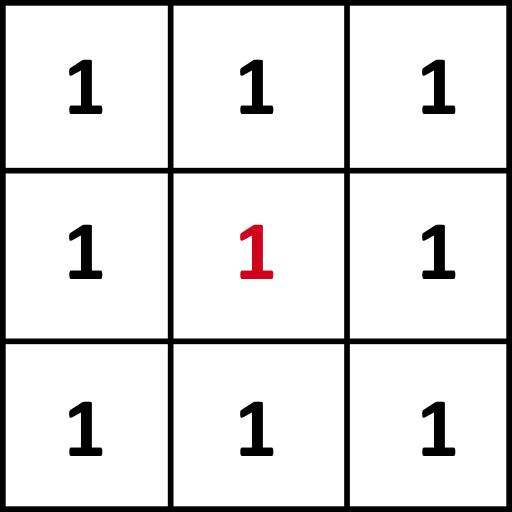
\includegraphics[width=4cm]{images/3x3kernel.jpg}
    \caption{Strukturni element dimenzija 3x3}
    \label{fig:kernel}
\end{figure}

Sam algoritam dilatacije je vrlo intuitivan i jednostavan za implementaciju. Iznad originalne slike postavi dani strukturni element, prikazan na slici \ref{fig:kernel}, te se iterira po pojedinom slikovnom elementu. Zatim, ukoliko se centralni element nađe iznad crnog slikovnog elementa originalne slike, na novoj slici se oboja u crno slikovni element koji se nalazi na koordinati na kojoj se nalazi centralni element te svih ostalih osam susjednih elemenata. Implementacija danog algoritma u programskom jeziku \emph{Java} prikazano je sljedećim izvornim kodom \citep{Gonzalez}.
\lstset{language=Java, tabsize=2}
\begin{lstlisting}
public BufferedImage applyFilter(BufferedImage sourceImage) {
    width = sourceImage.getWidth();
    height = sourceImage.getHeight();
    
    BufferedImage filteredImage = clone(sourceImage);
    for (int i = 0; i < width; i++) {
        for (int j = 0; j < height; j++) {
            int color = ImageUtilities.
                    getRed(sourceImage.getRGB(i, j));
            if (color == BLACK) {
                convolve(i, j, sourceImage);
            }
        }
    }
    return filteredImage;
}
// Konvoluiraj sliku strukturnim elementom
private void convolve(int i, int j, BufferedImage sourceImage, BufferedImage filteredImage) {
    for (int x = i - 1; x <= i + 1; x++) {
        for (int y = j - 1; y <= j + 1; y++) {
            if (x >= 0 && y >= 0 && x < width && y < height) {
                int rgb = ImageUtilities.
                        colorToRGB(255, 0, 0, 0);
                filteredImage.setRGB(x, y, rgb);
            }
        }
    }
}
\end{lstlisting}

Prikaz rada algoritma dilatacije vidljiv je na slici \ref{fig:dilation_good_example}. Bitno je primijetiti kako dano slovo ima sitnu nepravilnost u prednjem planu te bi ta nepravilnost dovela do velikih pogrešaka kod algoritma izvlačenja kostura slova, no dilatacija to uspješno rješava.
\begin{figure}[htb]
    \centering
    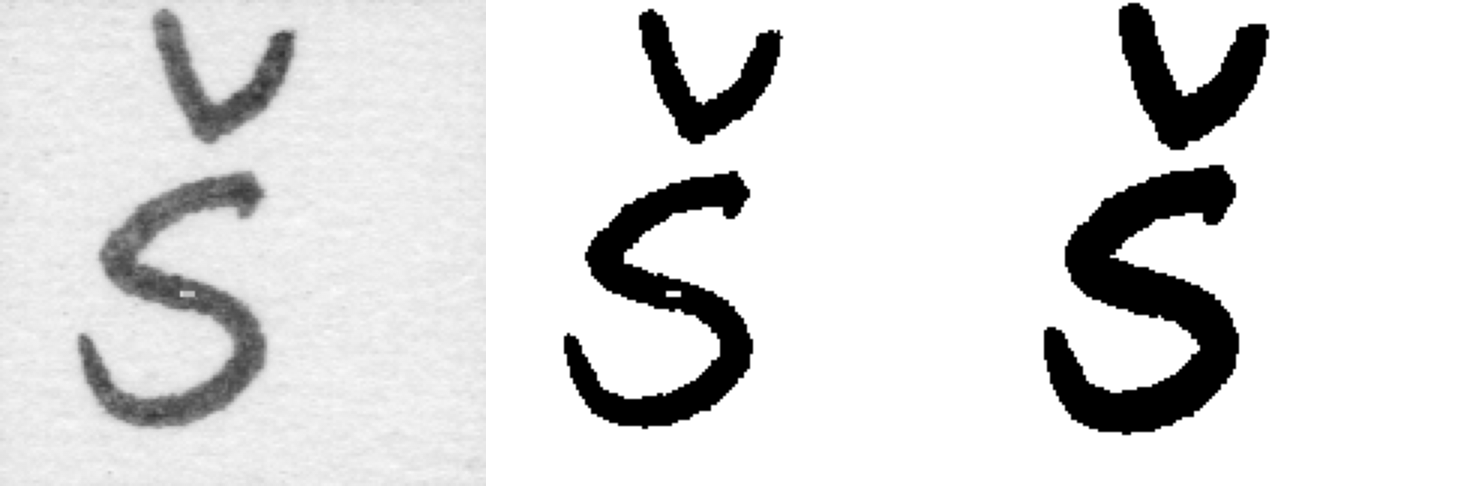
\includegraphics[width=10cm]{images/dilation_example.png}
    \caption{Prikaz rada algoritma binarizacije i dilatacije}
    \label{fig:dilation_good_example}
\end{figure}

Ukoliko dilatacija ne daje dobre rezultate u prvom prolazu, to jest još uvijek ostanu sitne praznine ili nepovezani dijelovi, može se ponoviti više prolaza. No time se gubi velika količina informacija o rukom pisanom slovu, što nikako nije poželjno.
\begin{figure}[htb]
    \centering
    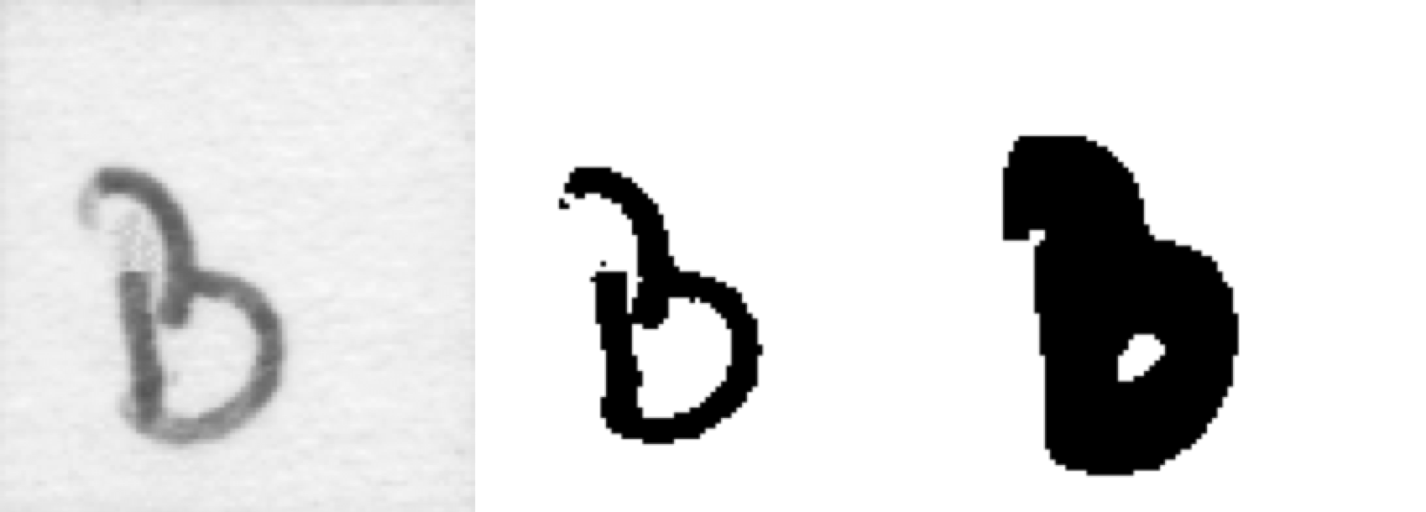
\includegraphics[width=10cm]{images/dilation_bad_example.png}
    \caption{Prikaz više prolaza algoritma dilatacije}
    \label{fig:dilation_bad_example}
\end{figure}
Dani problem se vidi na slici \ref{fig:dilation_bad_example} gdje je nakon tri prolaza algoritma dilatacije slovo 'B' neprepoznatljivo.

Sljedeći postupak je izvlačenje kostura slova, to jest stanjivanje \engl{thinning}.

\section{Stanjivanje}

Stanjivanje \engl{thinning} je jedna od osnovnih operacija u području matematičke morfologije. Poput dilatacije, obično se primjenjuje na binarnim (crno-bijelim) slikama, no postoje i verzije algoritma koje rade i za slike sivih nijansi. Operacija stanjivanja ima višestruku primjenu, no najčešće se koristi za izlučivanje kostura objekta, debljine jednog slikovnog elementa. U literaturi i na Internetu se stanjivanje i izlučivanje kostura vrlo često koriste kao sinonimi. Rezultat provedbe stanjivanja nad binarnom slikom je binarna slika.

U matematičko smislu, kao i kod dilatacije, stanjivanje je operacija nad skupom točaka koji pripadaju slici te skupom točaka koji provodi stanjivanje, to jest već prije spomenuti strukturni element. Jednostavan algoritam bi bio sljedeći: potrebno je uzeti u obzir sve slikovne elemente objekta, odnosno prednjeg plana, koji za susjeda imaju više od jednog slikovnog elementa koji pripada pozadini, zatim obrisati sve te elemente, ali samo u slučaju ukoliko neće doći do lokalnog razdvajanja objekta u dva dijela. Navedeni postupak ponavljati sve dok rezultat ne konvergira, to jest više se ne obriše niti jedan slikovni element u pojedinoj iteraciji algoritma. Ovaj postupak briše vanjske granice objekta, ali ne utječe na slikovne elemente na samim krajevima linija.

Navedeni algoritam se u morfologiji obavlja pomoću dva kvadratna strukturna elementa dimenzija $3 \times 3$, prikazanih na slici \ref{fig:thinning_el}, te svim njihovim rotacijama za 90 stupnjeva, što zapravo daje osam strukturnih elemenata. Element označen crvenom bojom predstavlja centralni element, to jest element kojim se vrši usporedba s originalnom slikom.
\begin{figure}[htb]
    \centering
    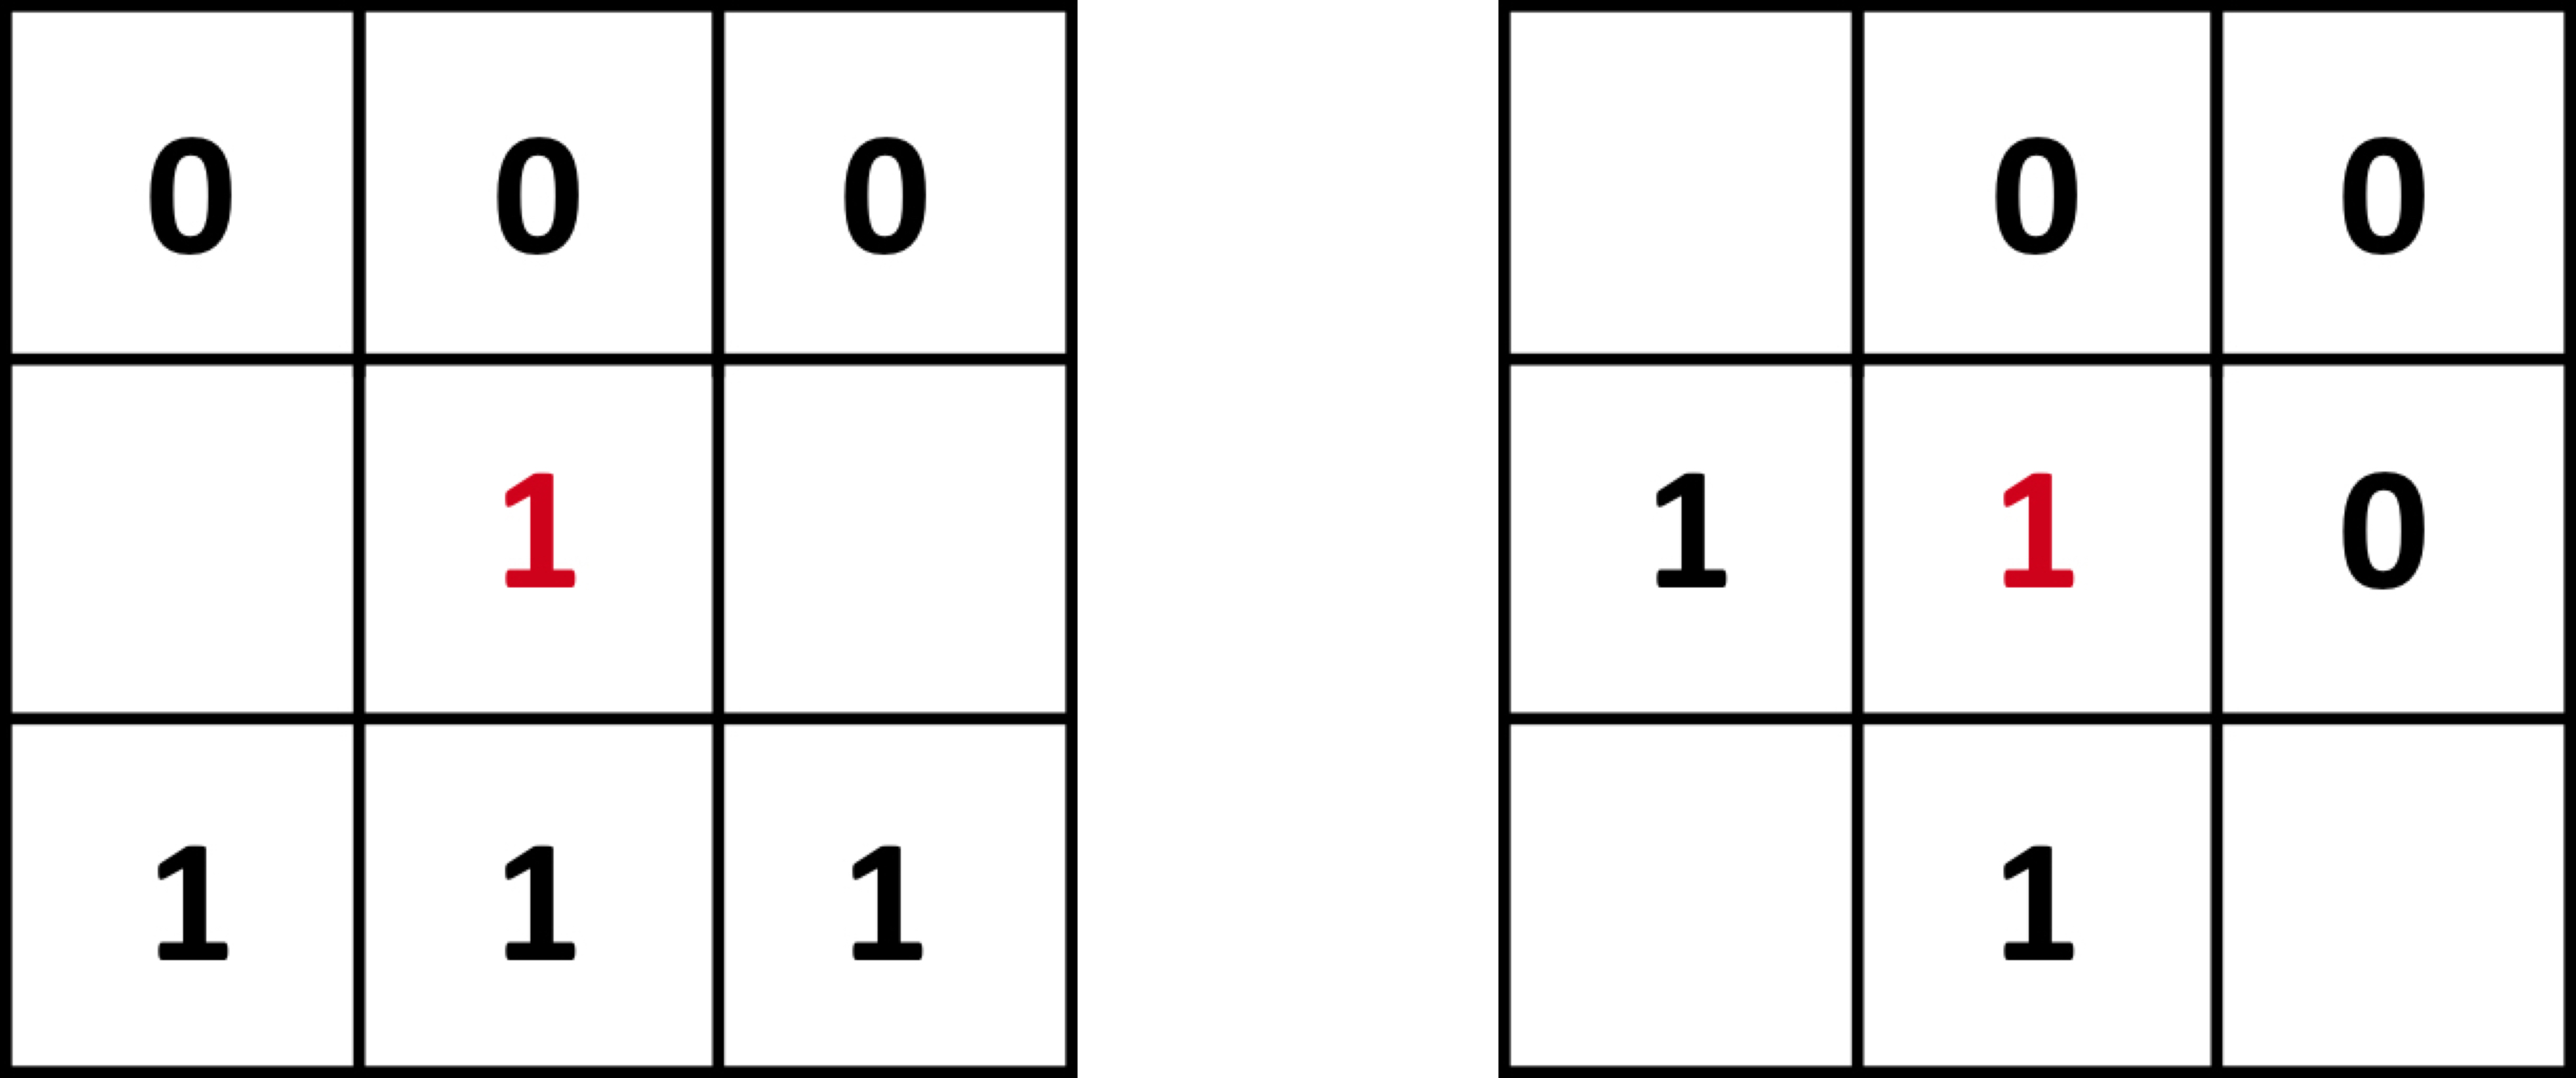
\includegraphics[width=10cm]{images/thinning_el.jpg}
    \caption{Strukturni elementi za stanjivanje}
    \label{fig:thinning_el}
\end{figure}

Navedeni algoritam nije pogodan za računalnu implementaciju što zbog kompliciranosti implementacije što zbog same brzine jer se praktički koristi osam strukturnih elemenata s kojima treba vršiti usporedbu. No Zhang i Suen su u svom radu \citep{Zhang-Suen}, davne 1984. predložili i opisali algoritam jednostavan za implementaciju na računalu. Princip ostaje isti, no umjesto osam strukturnih elemenata postoji samo jedan prikazan na slici \ref{fig:thinning_el_zhang}. Vrijednosti P na danom strukturnom elementu mogu poprimiti vrijednosti 0 ili 1, ovisno o tome je li slikovni element bijele ili crne boje, te se vrše izračunavanja u odnosu na susjedne slikovne elemente centralnom elementu, te unutar jedne iteracije postoje dvije pod-iteracije.

\begin{figure}[htb]
    \centering
    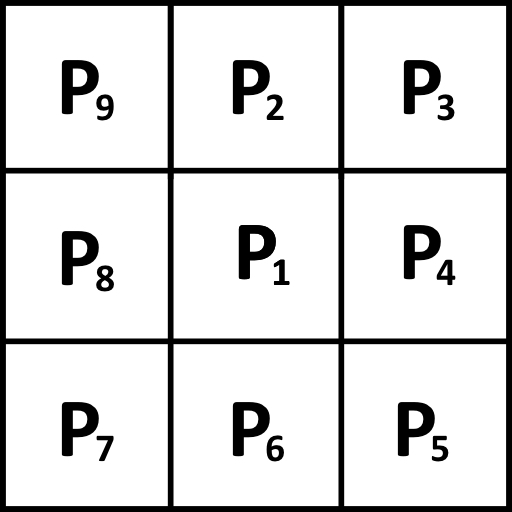
\includegraphics[width=4cm]{images/kernel.jpg}
    \caption{Zhang-Suenov strukturni element za stanjivanje}
    \label{fig:thinning_el_zhang}
\end{figure}

U prvoj pod-iteraciji, danim strukturnim elementom, briše se slikovni element na poziciji $P_1$ ukoliko su zadovoljeni sljedeći uvjeti:
\begin{gather} 
    2 \leq B(P_1) \leq 6, \\
    A(P_1) = 1, \\
    P_2\cdot P_4\cdot P_6 = 0 \  i\\ 
    P_4\cdot P_6\cdot P_8 = 0
\end{gather}
gdje je $A(P_1)$ broj '01' uzoraka u poretku $P_1, P_2, ...P_8, P_9$ i $B(P_1)$ broj crnih susjeda, to jest: 
\begin{gather} 
    B(P_1) = P_2 + P_3 + ... + P_8 + P_9.
\end{gather}
U drugoj pod-iteraciji mijenjanju se zadnja dva uvjeta u sljedeće:
\begin{gather} 
    P_2\cdot P_4\cdot P_8 = 0 \  i \\
    P_2\cdot P_6\cdot P_8 = 0,
\end{gather}
dok sve ostalo ostaje isto kao i u prvoj pod-iteraciji. Navedene iteracije se vrše naizmjence sve dok dana slika ne konvergira, to jest dok nakon zadnje iteracije više se ne obriše niti jedan slikovni element.

Na slici \ref{fig:thinning_good} prikazan je rad algoritma stanjivanja prema \emph{Zhang-Suenu}.
\begin{figure}[htb]
    \centering
    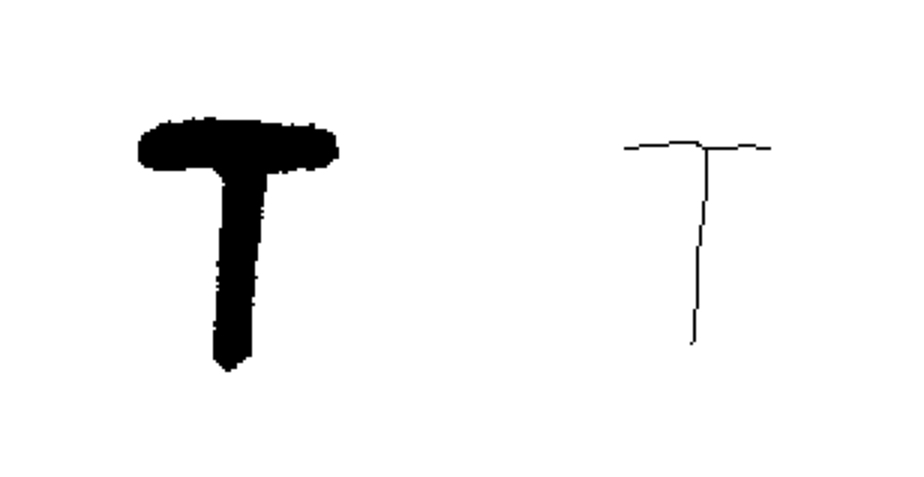
\includegraphics[width=8cm]{images/thinning_good.jpg}
    \caption{Stanjivanje prema \emph{Zhang-Suenu}}
    \label{fig:thinning_good}
\end{figure}

Na slici \ref{fig:thinning_bad} demonstriran je problem rada algoritma nad deformiranim objektom. Dakle, algoritam malu "rupicu" vidi kao pozadinu te oko nje gradi granice objekta, no tu u pomoć uskače dilatacija koja prikazanu nepravilnost ispuni.

\begin{figure}[htb]
    \centering
    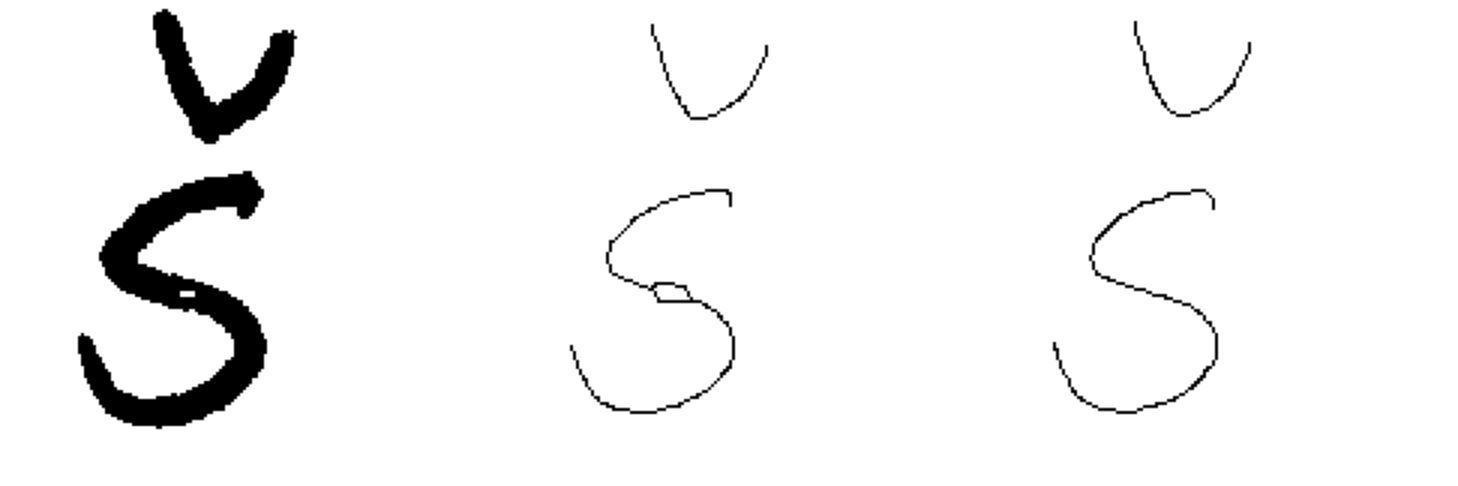
\includegraphics[width=12cm]{images/thinning_bad.jpg}
    \caption{Stanjivanje provedeno prije (srednja slika) i nakon (desna slika) dilatacije}
    \label{fig:thinning_bad}
\end{figure}

Implementacija iteracije prema \emph{Zhang-Suenu} u programskom jeziku \emph{Java} dana je sljedećim izvornim kodom.
\lstset{language=Java, tabsize=2}
\begin{lstlisting}
    private int[][] thinningIteration(Iteration iteration, int[][] inputImage) {
        int[][] marker = new int[width][height];
        for (int i = 1; i < width - 1; i++) {
            for (int j = 1; j < height - 1; j++) {
                int p2 = inputImage[i - 1][j];
                int p3 = inputImage[i - 1][j + 1];
                int p4 = inputImage[i][j + 1];
                int p5 = inputImage[i + 1][j + 1];
                int p6 = inputImage[i + 1][j];
                int p7 = inputImage[i + 1][j - 1];
                int p8 = inputImage[i][j - 1];
                int p9 = inputImage[i - 1][j - 1];

                int c1 = p2 == 0 && p3 == 1 ? 1 : 0;
                int c2 = p3 == 0 && p4 == 1 ? 1 : 0;
                int c3 = p4 == 0 && p5 == 1 ? 1 : 0;
                int c4 = p5 == 0 && p6 == 1 ? 1 : 0;
                int c5 = p6 == 0 && p7 == 1 ? 1 : 0;
                int c6 = p7 == 0 && p8 == 1 ? 1 : 0;
                int c7 = p8 == 0 && p9 == 1 ? 1 : 0;
                int c8 = p9 == 0 && p2 == 1 ? 1 : 0;

                int A = c1 + c2 + c3 + c4 + c5 + c6 + c7 + c8;
                int B = p2 + p3 + p4 + p5 + p6 + p7 + p8 + p9;
                int m1 = 0; int m2 = 0;
                switch (iteration) {
                    case ITERATION_FIRST:
                        m1 = (p2 * p4 * p6);
                        m2 = (p4 * p6 * p8);
                        break;
                    case ITERATION_SECOND:
                        m1 = (p2 * p4 * p8);
                        m2 = (p2 * p6 * p8);
                        break;
                }
                if (A == 1 && (B > 1 && B < 7) && m1 == 0 && m2==0)
                    marker[i][j] = 1;
            }
        }
        return outputImageFromMarker(inputImage, marker);
    }
\end{lstlisting}

\section{Segmentacija i skaliranje slova}

Posljednji korak pri obradi danog skupa podataka rukom pisanih slova je segmentacija i skaliranje pojedinog binarnog slova. Razlog tomu je postizanje invarijantnost pojedinog slova na dimenzije, što bi, ukoliko nije provedeno, kasnije predstavljalo problem prilikom klasifikacije pojedinog slova ukoliko su ista slova različitih dimenzija.

Prvi korak je segmentacija slova. Kako su već sva slova izdvojena s obrasca i pretvorena u crno-bijelu sliku algoritam je vrlo jednostavan. Dakle, potrebno je pronaći najmanji pravokutnik koji omeđuje slovo. Kako je slika crno-bijela, algoritam se svodi na pretraživanje \emph{x} vrijednosti najbližeg i najdaljeg crnog slikovnog elementa po visini slike, te \emph{y} vrijednosti za najbližeg i najdaljeg crnog slikovnog elementa po dužini slike, kako je prikazano na slici \ref{fig:crop_example}.
\begin{figure}[htb]
    \centering
    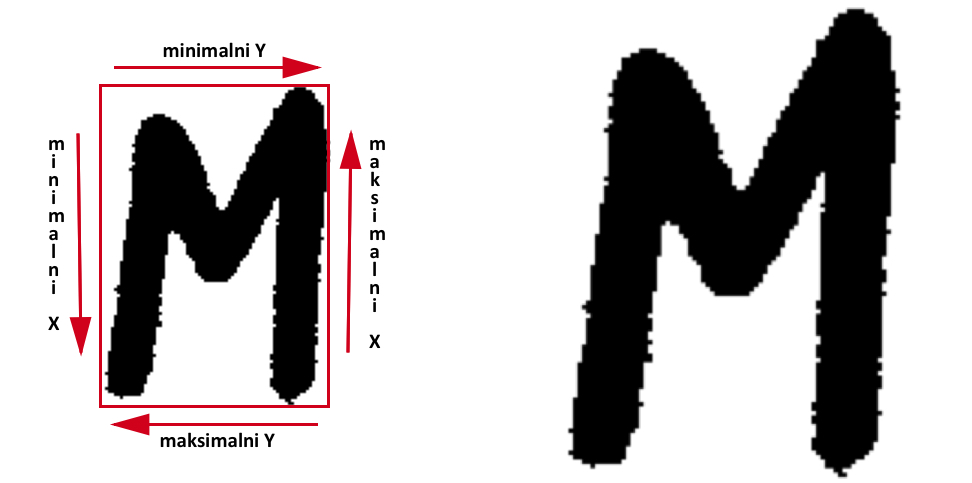
\includegraphics[width=12cm]{images/crop_example.jpg}
    \caption{Segmentacija slova}
    \label{fig:crop_example}
\end{figure}

Nakon segmentacije slijedi skaliranje izdvojenog slova. Za potrebe ovog rada sva izdvojena slova su skalirana na kvadratne dimenzije $30 \times 30$. Kod skaliranja slike postoji više načina i pristupa, no neki od poznatijih su bilinearna i bikubična interpolacija koje pokušavaju sačuvati glatkost slike. No kako je slika slova binarna, to jest crno-bijela, bilinearna ili bikubična interpolacija bi napravila više štete nego koristi jer bi aproksimacijom slikovnog elementa rezultat mogao biti iz područja sive boje, dakle više ne bi bila binarna slika te bi opet trebalo obaviti binarizaciju. Stoga je za potrebe ovog rada korištena metoda najbližeg susjeda.

\begin{figure}[htb]
    \centering
    
\includegraphics[width=8cm]{images/resize_example.jpg}
    \caption{Skaliranje slova}
    \label{fig:resize_example}
\end{figure}

Prilikom uvećavanja slike u slici nastaju praznine, kod metode najbližeg susjeda, kako joj i ime kaže, uzima se vrijednost najbližeg slikovnog elementa te se postavlja na trenutnu prazninu. Nema interpolacije više vrijednosti, pa će binarna slika ostati binarna. Kod smanjivanja slike princip je isti, samo što umjesto popunjavanja praznina slijedi izuzimanje slikovnog elementa te se uzima samo onaj najbliži. Prikaz rada algoritma vidljiv je na slici \ref{fig:resize_example}. Bitno je napomenuti da je metoda najbližeg susjeda najjednostavnija te da bi se pri obradi slike u boji trebala izbjegavati i koristiti neku od već gore spomenutih.

Za potrebe ovog rada segmentacija i skaliranje slova se zbivala nakon binarizacije slike, te se nakon toga po potrebi odvijala dilatacija, pa zatim stanjivanje prednjeg plana. Implementacija skaliranja slike metodom najbližeg susjeda u programskom jeziku \emph{Java} dana je sljedećim izvornim kodom.
\lstset{language=Java, tabsize=2}
\begin{lstlisting}
    public BufferedImage applyFilter(BufferedImage sourceImage, int newWidth, int newHeight) {
        int width = sourceImage.getWidth();
        int height = sourceImage.getHeight();
        BufferedImage scaledImage = new BufferedImage(
                newWidth, newHeight, sourceImage.getType());
        float xRatio = width / (float) newWidth;
        float yRatio = height / (float) newHeight;
        int x, y;
        for (int i = 0; i < newWidth; i++) {
            for (int j = 0; j < newHeight; j++) {
                x = (int) Math.floor(i * xRatio);
                y = (int) Math.floor(j * yRatio);
                scaledImage.setRGB(i, j, sourceImage.getRGB(x, y));
            }
        }
        return scaledImage;
    }
\end{lstlisting}